\documentclass[10pt]{article}

\RequirePackage{nybohansenPreamble}

\usepackage[draft]{fixme}
\newcommand{\authorName}{Mads Ohm Larsen and Kasper Nybo Hansen}
\newcommand{\authorEmail}{\{omega, nybo\}@diku.dk}
\newcommand{\titleName}{Project 2}
\newcommand{\courseName}{Advanced Algorithms 2011}

\author{\authorName \\\texttt{\small{\authorEmail}}}
\title{\textsc{\titleName \\ \courseName}}
\makeindex

\begin{document}
\maketitle    

\section*{Question 1.1} % (fold)
\label{sec:question_1_1}
\paragraph{Part A} % (fold)
\label{par:part_a}

We are given a complete undirected graph $G = (V,E)$, with non-negative weights $d_{ij}$, and a viewing distance $d$. The problem is to find the shortest simple cycle so each vertex ($v_i$) is either seen or visited.

In the following we assume that the couple only wishes to visit a monument once, but possible see it multiple times. I.e. each node is visited at most once, and the cycle is thus a simple cycle. We can define the problem as follows

\begin{mydef}
Given a graph $G = (V, E)$ let a shortest cycle consist of the path $p = \{v_0, v_1,v_2,...,v_n, v_0\}$, where $v_i \in V$. Let 
\begin{equation}
  v(i) = \{j  \in V | d_{ij} \leq d\}
\end{equation}
be the set of vertices in the vicinity of vertex $i$. Let the distance between two vertices, $v_i$ and $v_j$, be calculated as
\begin{equation} 
D(v_i,v_j) = 
\begin{cases}
 d_{ij} &  \quad d_{ij}>d \\
 0      &  \text{otherwise}
\end{cases} 
\end{equation} 

The path $p$ should be chosen so 
\begin{equation}
  \forall v \in V : \exists v_i \in p : v \in v(v_i) 
\end{equation}        

The vertices in $p$ and their ordering should be chosen so the following function is minimized
\begin{equation}
  D(p[0],p[n])+\sum_{i=0}^{n-1} D(p[i],p[i+1])
\end{equation}

where $p[i]$ is the $i'th$ vertex in the path $p$.
\label{def1}
\end{mydef}

Transforming the above definition into a decision problem yields: Given a graph $G$ and a number $l$ is there a cycle of length at most $l$, which satisfy the above.

The corresponding language is

\begin{align*}
   \text{TCP_cycle} = \{ \langle G, l \rangle : &G = (V,E) \text{ complete undirected graph},\\ 
                                               &l = \text{Length of tour}  \}
\end{align*}

% paragraph part_a (end)

\paragraph{Part B} % (fold)
\label{par:part_b}
We need to show that the TCP problem is NP-complete. In order tho show that the TCP problem is NP-complete, we need to show that $TCP \in NP$ and to show that it is complete we show that $HAM-CYCLE \leq TCP$.

We can show this, by utilizing that we know that the Hamilton cycle is NP-complete. If we can come up with a polynomial time algorithm, that can transform an instance $\alpha$ of the TCP problem into an instance $\beta$ of the Hamilton cycle and yield the same results, we can show that TCP is NP-complete.

\fxnote{Hvis $d=0$ er problemet blot et \textsc{HAM-CYCLE} problem}
\fxnote{Hvis $d>0$ er problemet ...}

% paragraph part_b (end)
% section question_1_1 (end)

\section*{Question 1.2} % (fold)
\label{sec:question_1_2}
% Tror måske det kan gøres således:
%    A - B
%     \ /
%      C
% Den korteste TCP cycle er A (eller B eller C), men det mindste 1-tree indeholder alle knuderne

\begin{figure}
	\centering
	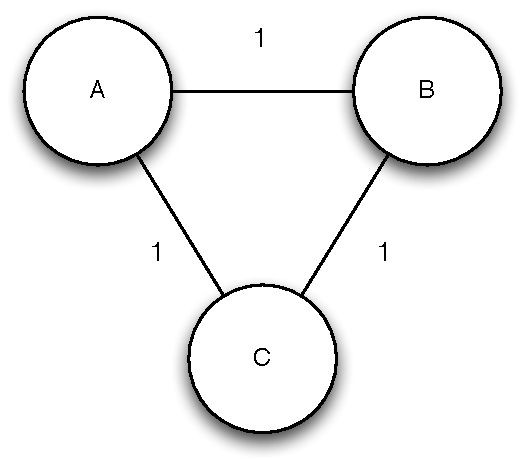
\includegraphics[width=0.4\textwidth]{figures/unicycle.pdf}
	\caption{A graph where the smallest 1-tree is larger than the optimal TCP cycle. $d \geq 1$}
	\label{unicycle}
\end{figure}
In figure \ref{unicycle} we have depicted a set of points $A$, $B$ and $C$, in which the smallest 1-tree, $A-B-C$ is larger than the optimal TCP cycle, which can be one of the three points.
The $d$ value is in this instance greater or equal to $1$.
% section question_1_2 (end)

\section*{Question 1.3} % (fold)
\label{sec:question_1_3}
First lets define the function $v(i)$ to be
\begin{equation}
   v(i) = \{ j \in V\ |\ d_{ij} < d \}
\end{equation}

% In the following \texttt{ILP} definition of the problem, $x_{ij}$ denotes the usage of an edge from $i$ to $j$, however, this does not mean that the edge from $j$ to $i$ is used.
% 
% The weight $d_{ij}$ is the same as $d_{ji}$.
% 
% \begin{align}
% \min &\qquad \sum_{i=1}^{n-1} \left( \sum_{j=i+1}^{n} d_{ij} \left( x_{ij} + x_{ji} \right) \right) \nonumber\\
% s.t. &\qquad  y_i = 1 \quad \text{if } \forall j \in V \setminus i\ |\ i \notin v(j) \nonumber\\
%      &\qquad \sum_{j=1}^{n} y_j \left( x_{ij} + x_{ji} \right) = 2 \quad \text{if $y_i = 1 \land \sum_{j=1}^n y_j \geq 2$}  \nonumber\\
%      &\qquad y_i \in \{0,1\}, \quad x_{ij} \in \{0,1\} \nonumber
% \end{align}

In the following \texttt{ILP} definition of the problem, $x_{ij}$ denotes the usage of an edge from $i$ to $j$.
Likewise, $y_i$ denotes the usage of vertex $i$.
\begin{align}
\min &\qquad \sum_{(i,j) \in V \times V} d_{ij} x_{ij} \nonumber\\
s.t. &\qquad y_i = 1 \quad \text{if } \forall j \in V \setminus i\ |\ i \notin v(j) \quad \forall i \in V \nonumber\\
     &\qquad \sum_{j \in V} x_{ij} \geq y_i \quad \text{if } \sum_{i \in V} y_i \geq 2 \quad \forall i \in V \nonumber\\
     &\qquad \sum_{(i,j) \in V \times V} x_{ij} \geq \sum_{i \in V} y_i - 1 \nonumber\\
	 &\qquad y_i \in \{0,1\}, \quad x_{ij} \in \{0,1\} \nonumber
\end{align}


\fxnote{Hvis vi besøger en vertex vi har set før, så ser vi faktisk monumentet 2 gange. Dette strider imod den initielle antagelse. Måske vi skal fjerne den, således et monument kan besøges flere gange?}

\fxnote{Tekstforklaring på de 3 led i \TeX-fil}
% Første led:
% 	Knuden er med, hvis der for alle $j$ i V gælder at $i$ ikke er i nærheden af nogen af dem

% Andet led:
% 	Hvis der er mere end to knuder "aktive" skal der være mindst 1 kant gående fra de "aktive" knuder til andre knuder (etv. andre aktive)
% 	Denne forhindre at der kommer hop i knuderne, da alle "aktive" knuder nu vil have mindst en kant

% Tredje led:
% 	Antallet af "aktive" kanter er større end eller lig med antallet af "aktive" knuder minus 1
% 	Denne sørger for at grafen er sammenhængende
% 
% Hmmm....
% Nederen, troede ellers lige at den var der.
% Følgende er dog modeksempel for at den ikke bliver sammenhængende
%     A
%   /   \
%  B --- C
% 
%  D --- E
%   \   /
%     F
% section question_1_3 (end)

\section*{Question 1.4} % (fold)
\label{sec:question_1_4}

% section question_1_4 (end)

\section*{Question 2.1} % (fold)
\label{sec:question_2_1}

% section question_2_1 (end)

\section*{Question 2.2} % (fold)
\label{sec:question_2_2}

% section question_2_2 (end)

%\section*{Question 2.3} % (fold)
%\label{sec:question_2_3}
% Optional
% section question_2_3 (end)


%\bibliographystyle{abbrv}
%\bibliography{bibliography}

\end{document}                      



